\setchapterimage[8.5cm]{palomar}
\setchapterpreamble[u]{\margintoc}
\chapter{The Zwicky Transient Facility (ZTF)}
\labch{ztf}
\begin{fquote}[Fritz Zwicky][Catalogue of selected compact galaxies and of post-eruptive galaxies][1971]I soon became convinced, however, that all theorizing would be empty brain exercise and therefore a waste of time unless one first ascertained what the population of the universe really consists of, how its various members interact and how they are distributed throughout cosmic space.
\end{fquote}

The second experiment heavily utilised for the work of this thesis was the \emph{Zwicky Transient Facility} (ZTF), a `48-inch' telescope located on Mount Palomar, California. ZTF had first light in October 2017, with full survey operations beginning in March 2018. In the following chapter, the telescope itself and the ZTF data analysis chain are introduced.

\section{The ZTF Telescope}

The central design philosophy of ZTF was to \emph{maximise volumetric survey speed at fixed cost}, where volumetric survey speed describes the volume of universe observed to some absolute magnitude per unit time \sidecite{ztf_system}. Optimising volumetric survey speed requires a careful balancing of system overheads (how much time is spent preparing for an exposure), field of view (how much sky area is imaged in each exposure), and the limiting magnitude (heavily influenced by how long each exposure lasts). Maximising this quantity will then ultimately maximise the rate of optical transient detections, a key science goal of ZTF \sidecite{ztf_19_science}. This principle has guided the development of telescope hardware introduced in the following subsections.

\subsection*{Telescope Structure}

ZTF is the latest in a long line of instruments using the \emph{Samuel Oschin Telescope} \cite{ztf_system}, a Schmidt telescope located at the Palomar Observatory in California  \sidecite{harrington_52}. The Schmidt design is a common class of telescope using a curved lens known as a \emph{Schmidt corrector plate} alongside a reflecting mirror, with a curved focal plane lying within the telescope tube \sidecite{schmidt_32}. This basic design is illustrated in Figure \ref{fig:ztf_schematic}, with the golden arrows indicating the path of light. The Samuel Oschin Telescope has a 48-inch (1.2m) diameter aperture, with light focussed by the lens system and then reflected by the 1.8m primary mirror onto the ZTF camera \sidecite{ztf_obs_system}. In addition to the Schmidt Corrector plate, an additional \emph{trim plate} lens was added for the ZTF telescope, alongside additional optical elements in the camera itself. To reduce stray reflected light reaching the camera, the telescope also has a number of \emph{baffles} \cite{ztf_obs_system}. These are aluminium rings coated in non-reflecting black paint, distributed along the telescope length. 

\begin{figure}[!ht]
	\centering 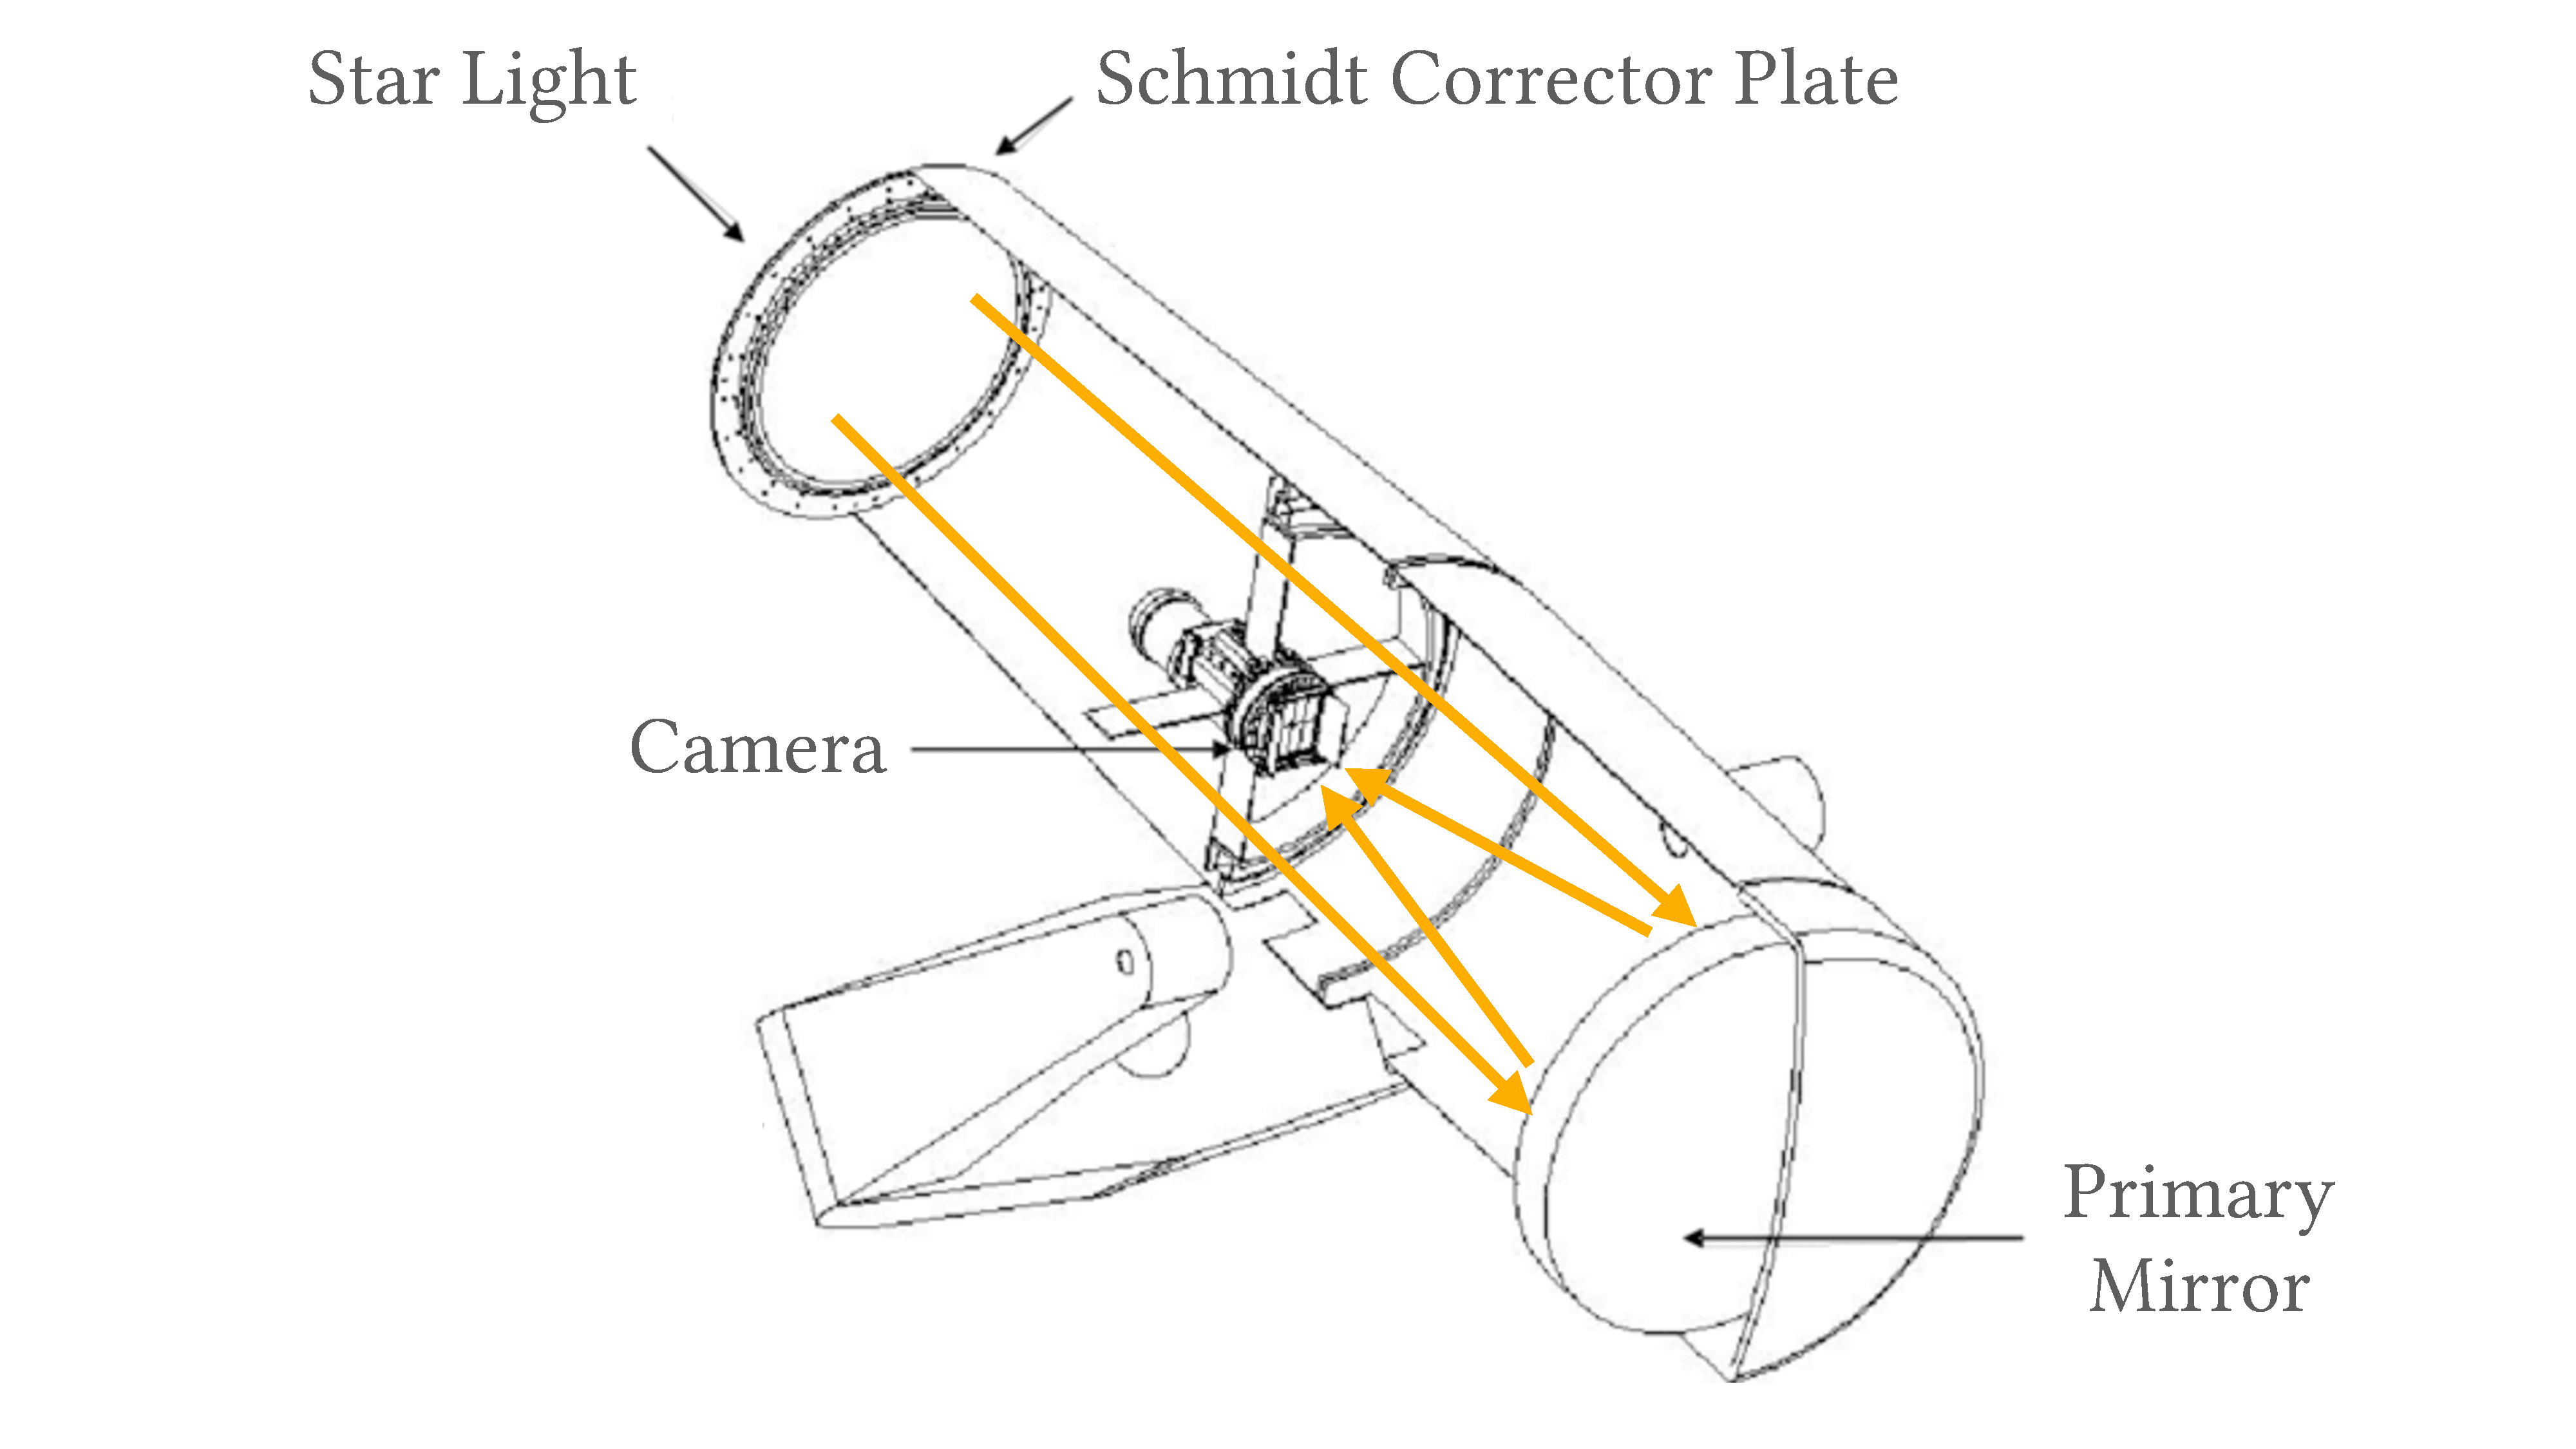
\includegraphics{ZTF/telescope_schematic}
	\caption{Overview of the basic Schmidt telescope design, adapted from \cite{quest_07}. The golden arrows indicate light paths.}
	\label{fig:ztf_schematic}
\end{figure}

The telescope can be rotated rapidly to point to different \emph{fields} (pre-defined on a static grid), with the time to slew between adjacent fields (separated by $\sim$7 degrees) being less than the time required to read out the camera data between exposures \cite{ztf_system}. The slewing process thus provides negligible additional overhead time. It is also entirely automated, with a dedicated robotic observing system executing the schedule for a given night. 

The telescope system also includes a robotic shutter which can open or close in <0.5s \cite{ztf_system}, with typical exposures then lasting 30s but extending up to 300s for certain observing modes. Before illuminating the ZTF camera, reflected light first passes through an optical filter. ZTF has three filters (ZTF-g, ZTF-r and ZTF-i) which are stored outside the telescope tube when not mounted, as well as a robotic arm that can exchange the mounted filter with an overhead time of $\sim$100s \cite{ztf_system}. Observations are typically conducted on the same field with multiple filters on a given night, providing colour information for detected objects.

The Schmidt design has the drawback that the camera itself blocks part of the telescope tube ($\sim$20\% for ZTF \cite{ztf_obs_system}), leading to a reduction in light throughput. To minimise this obscuration, the ZTF camera is suspended inside the telescope tube by a three-vane instrument spider, rather than e.g the four-vane spider design shown in Figure \ref{fig:ztf_schematic}.  Schmidt telescopes also have curved focal planes, so ZTF includes additional corrective optics. The camera system itself is also effectively `curved', with each of the 16 constituent pixel blocks having a unique tilt towards the focal plane \cite{ztf_system}. Ultimately, the telescope field of view spans 7.3\arcdeg (N-S) x 7.5\arcdeg (E-S) \cite{ztf_obs_system}, yielding a 55 sq. deg. area for each field. The complete process for a 30s exposure, including slewing, observation and data readout, can be completed in just 38.3s  \cite{ztf_system}. The entire ZTF system can be seen in Figure \ref{fig:ztf_diagram}.

\begin{figure}[!ht]
	\centering 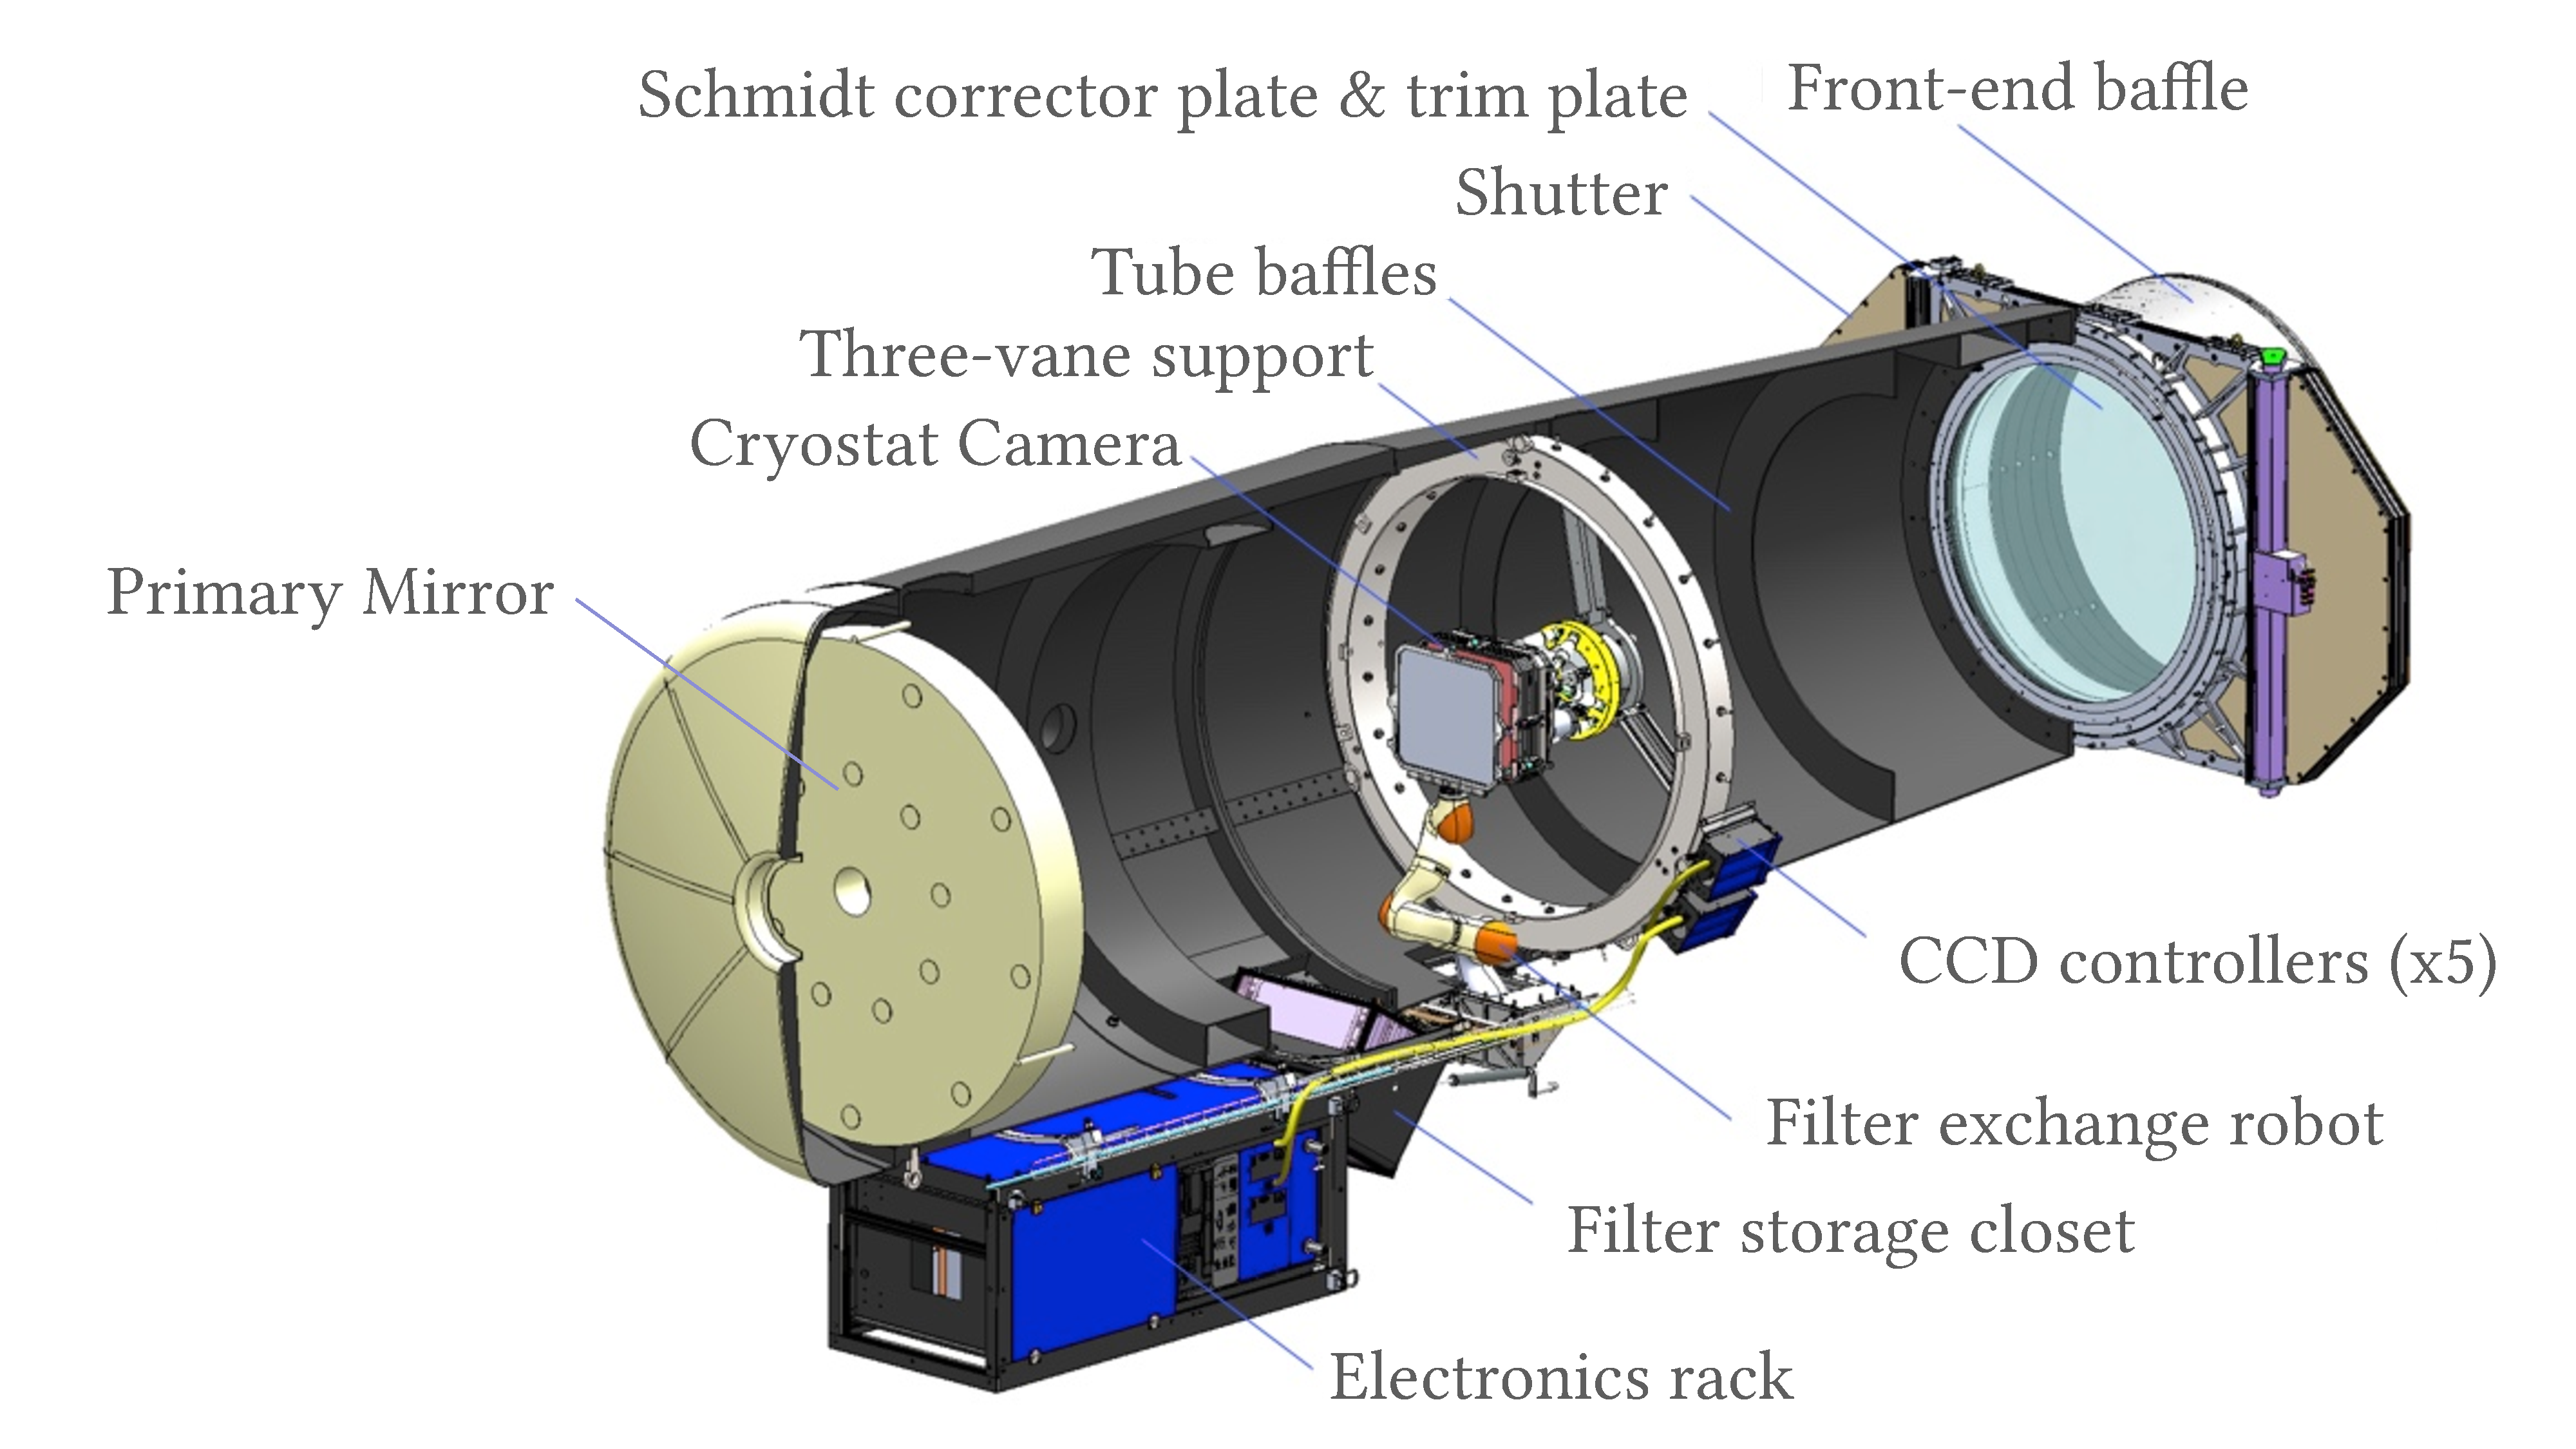
\includegraphics{ZTF/ztf_full}
	\caption{Overview of the ZTF telescope, adapted from \cite{ztf_obs_system}.}
	\label{fig:ztf_diagram}
\end{figure}

\subsection*{Camera}

The ZTF camera is constructed from \emph{charge-coupled devices} (CCDs). CCDs are semiconductors which store charge in potential wells that can be moved spatially, a property that is well-suited to high-resolution imaging \sidecite{boyle_70}. Incident photons transfer energy to electrons within the semiconductor, liberating charge in a process similar to the \emph{photoelectric effect} \sidecite{carroll_06, einstein_photoelectric_1905}. CCD pixels can be constructed which collect charge during an exposure, and these pixels can then be read out. Measuring the charge accumulated in a pixel over an exposure then provides a measurement of the integrated light incident on that pixel. The conversion efficiency from photons to detected electrons in a pixel is known as the \emph{quantum efficiency} (QE), and for CCDs is often $\gtrsim$80\%. 

The ZTF camera, shown in Figure \ref{fig:ztf_camera}, is composed of 16 separate CCD `wafers', each of which contains $\sim$6k x 6k pixels. The central 8 wafers employ a double-layer coating to boost QE, while the remainder have a single-layer anti-reflective coating, explaining the visible colour difference in Figure \ref{fig:ztf_camera}.

\begin{marginfigure}
	\centering 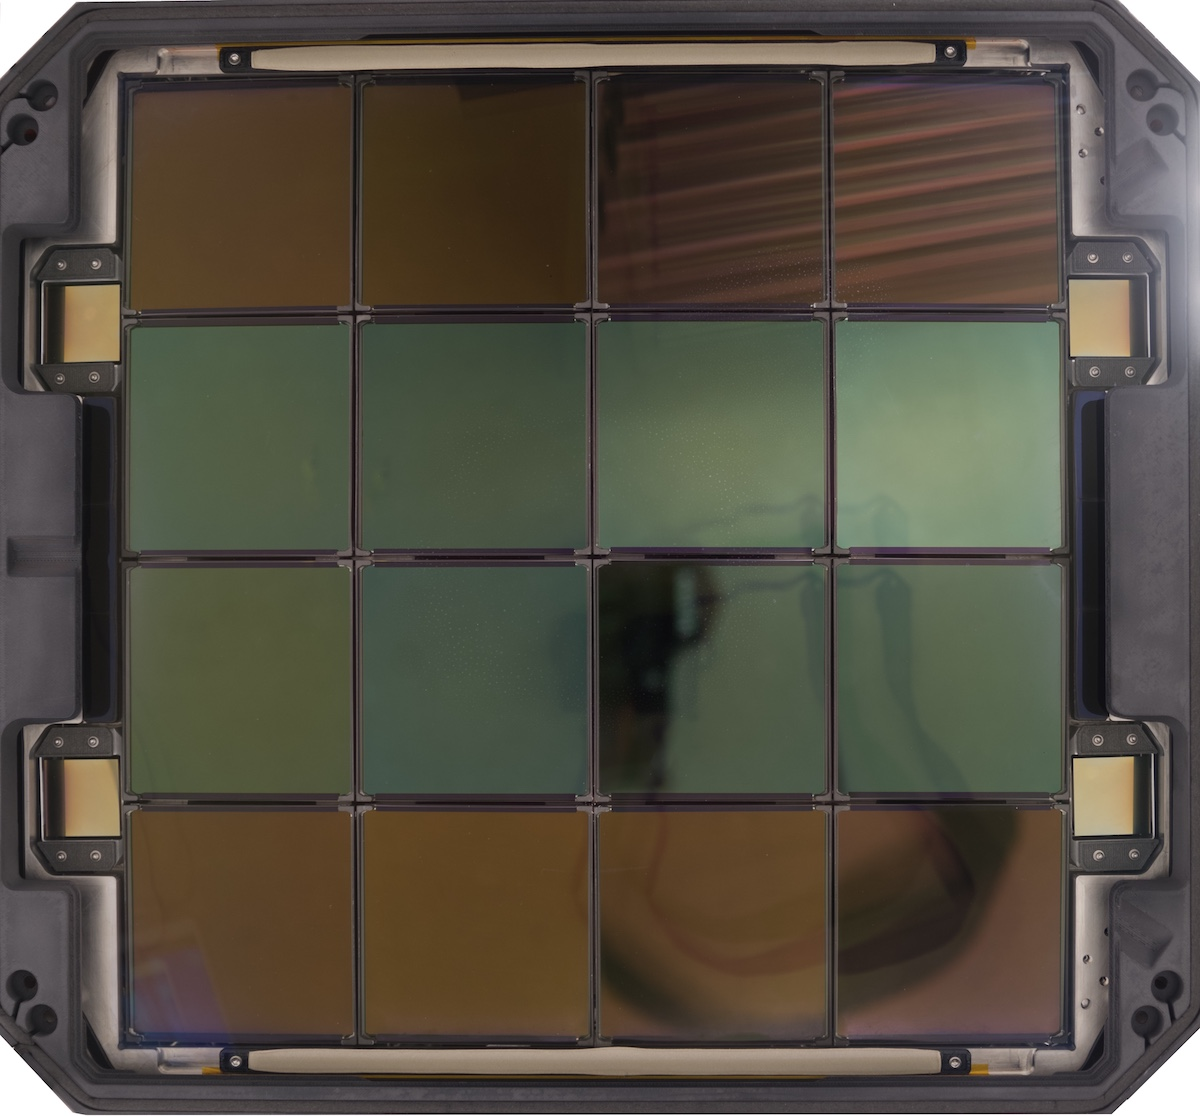
\includegraphics{ZTF/ztf_fp_med}
	\caption{An image of the ZTF camera, from \cite{ztf_system}.}
	\label{fig:ztf_camera}
\end{marginfigure}

These science CCDs are mounted on a cold plate within a temperature-controlled vacuum \emph{cryostat} \cite{ztf_obs_system}. Light enters through a curved vacuum window which additionally serves as a lens. Each individual CCD then has an additional field flattener lens and is mounted with a unique tilt towards the focal plane. Within the cryostat the cold plate temperature is maintained at 165K, with $\sim$1K variations across the plate, while the CCD temperature is maintained at 170K. 

The corresponding CCD efficiency at these temperatures can be seen in Figure \ref{fig:ztf_qe}, colour-coded for the single-layer-coated CCDs (grey) and the double-layer-coated CCDs (green). The filter transmission for the ZTF-g, ZTF-r and ZTF-i filters are shown in blue, orange and red respectively. For g and r, QE remains above 80\% in the relevant 400-700nm rage for all CCDs, rising to $\gtrsim$90\% for the double-coated central CCDs. For i, there is a somewhat lower range of $\sim$80\% to $\sim$40\% across the band.

\begin{marginfigure}
	\centering 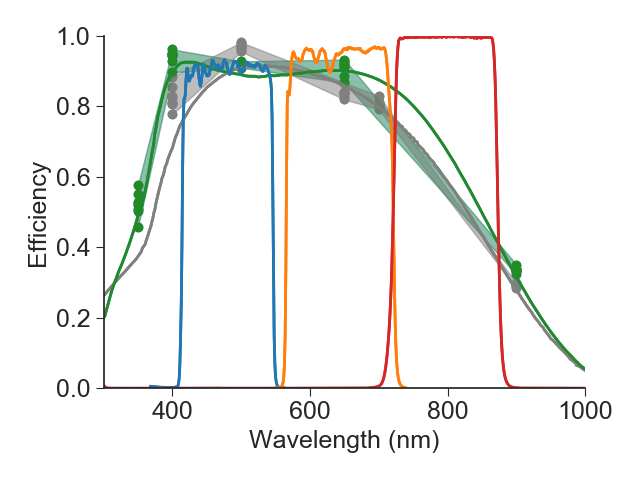
\includegraphics{ZTF/QE_curves_delivered}
	\caption{The quantum efficiency of ZTF CCDs, from \cite{ztf_system}.}
	\label{fig:ztf_qe}
\end{marginfigure}

There are also four additional CCDs with $\sim$2k x 2k pixels, embedded outside the central camera, which can be seen in Figure \ref{fig:ztf_camera}. One of these outer CCDs acts as a guiding camera, to ensure pointing accuracy by identifying the position of reference stars. The remaining CCDs each have a differently offset from the camera, and are collectively used to infer the extent of optical aberrations from atmospheric turbulence \sidecite{tokovinin_06}. The entire cryostat structure is shown in Figure \ref{fig:cryostat_exploded}.

\begin{figure*}
	\centering 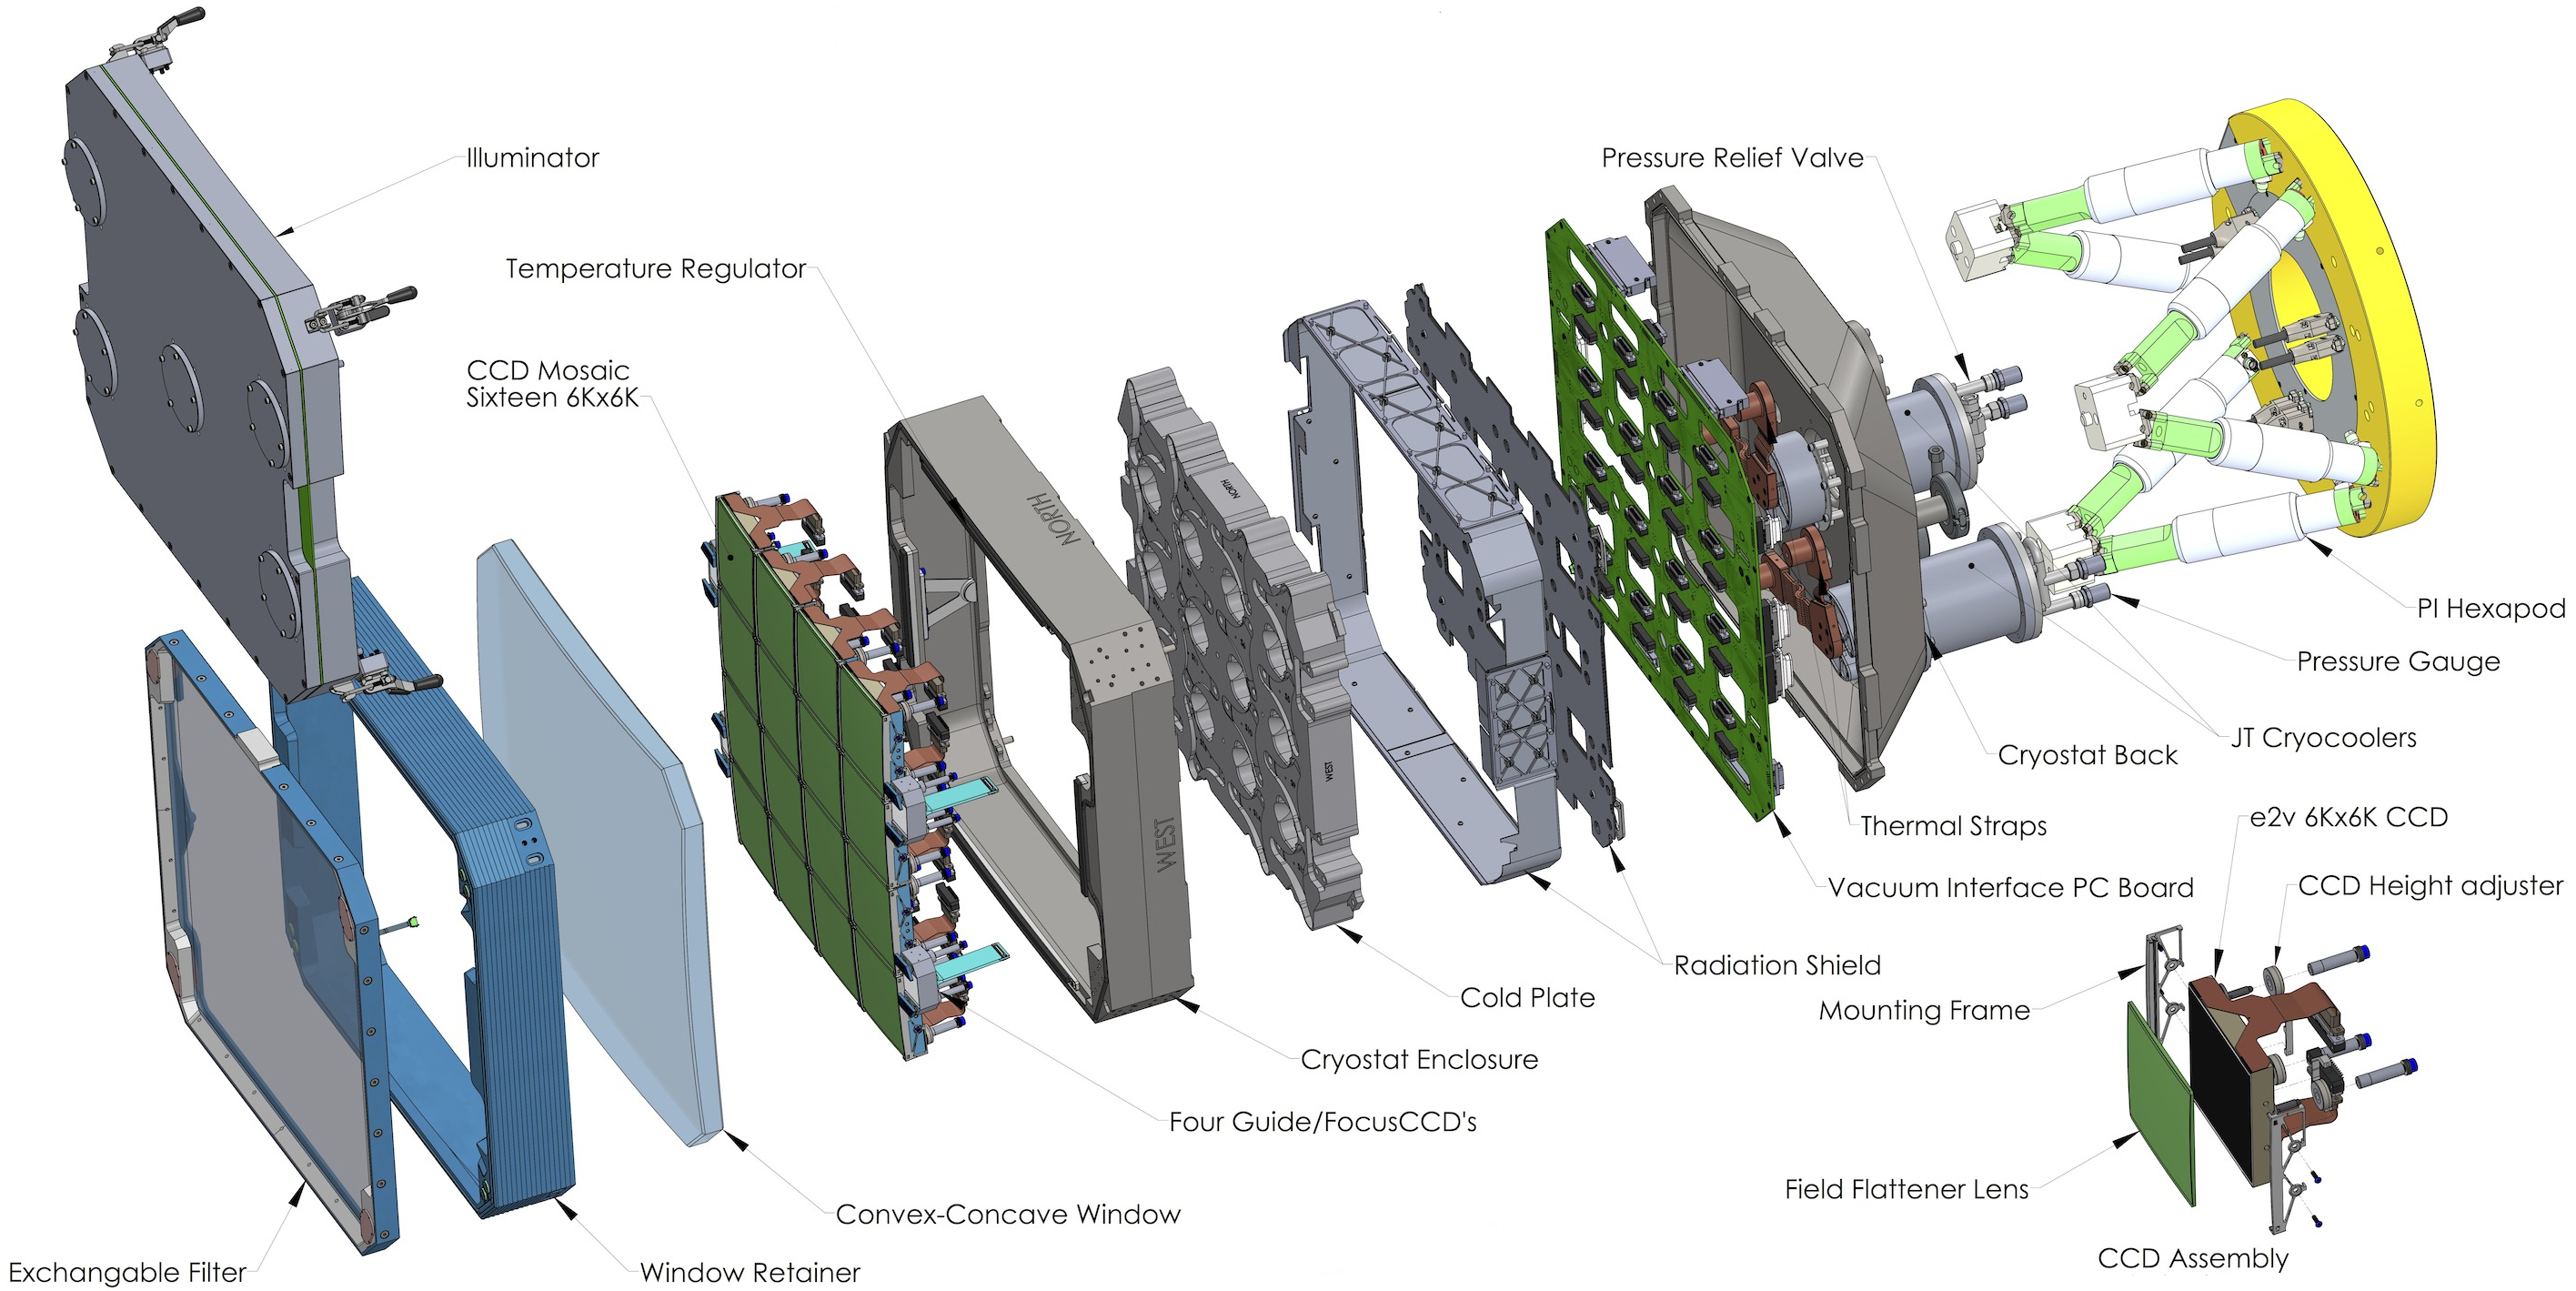
\includegraphics{ZTF/cryostat_exploded}
	\caption{The ZTF cryostat design, from \cite{ztf_system}.}
	\label{fig:cryostat_exploded}
\end{figure*}

Each CCD is split into four distinct quadrants, with each of these 64 quadrants then having an independent set of readout electronics. Gaps between the camera CCDs give an instrumented focal plane fill factor of 86.7\%, thus yielding a 47.6 sq. deg field of view for each ZTF exposure. This can be seen in Figure \ref{fig:ztf_footprint}, with the predecessor PTF/iPTF camera and other surveys provided for comparison. The moon and nearby galaxy Andromeda are also shown for scale.

\begin{figure*}
	\centering 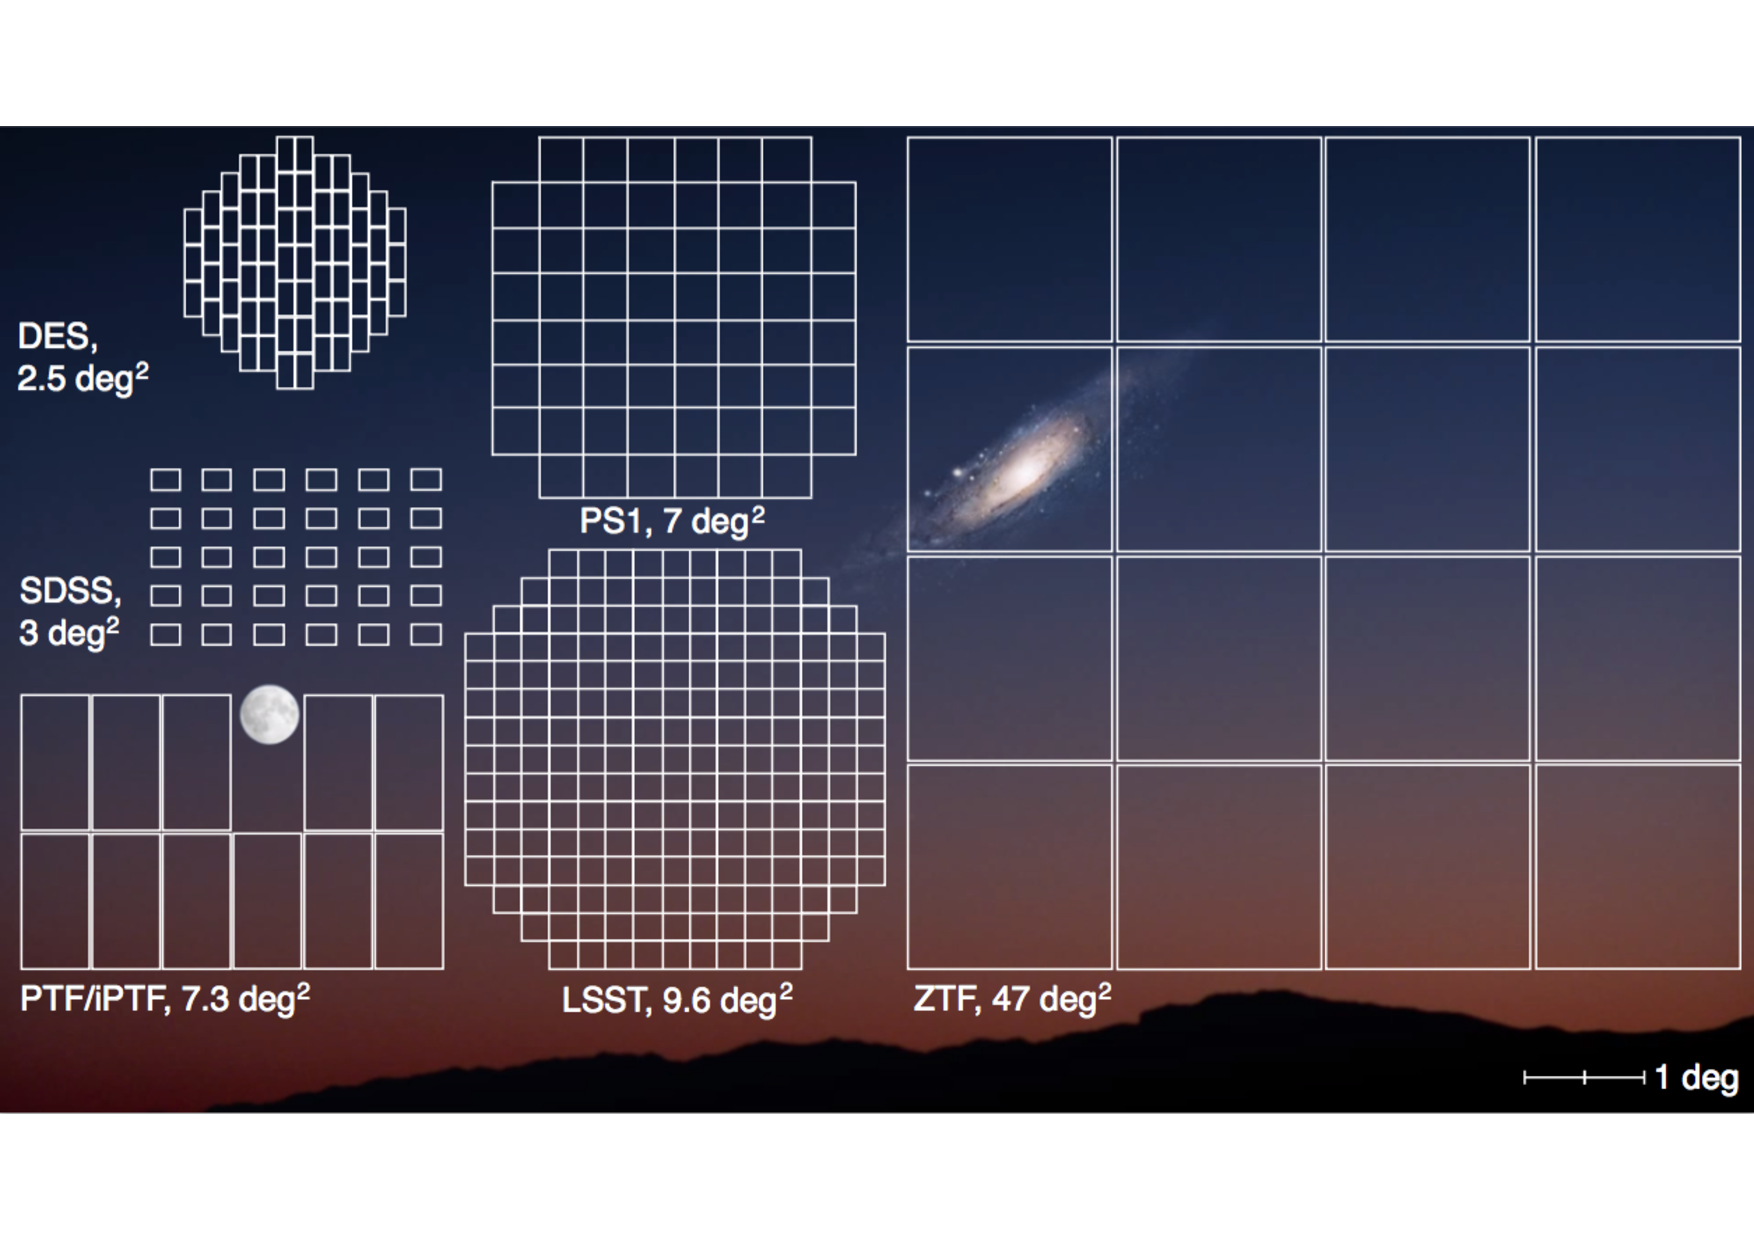
\includegraphics{ZTF/fov}
	\caption{The ZTF camera footprint, from \cite{laher_18}.}
	\label{fig:ztf_footprint}
\end{figure*}

\section{ZTF Scheduling and Surveys}
\label{sec:survey}

ZTF observations are handled within the framework of a \emph{primary grid}, with which the sky is divided into a grid of pre-defined \emph{fields}. This primary grid covers 87.5\% of the accessible sky once camera chip gaps are accounted for \sidecite{ztf_survey_19}. There is also a \emph{secondary grid}, offset diagonally from the primary grid to minimise chip gap overlap, yielding a combined 99.2\% coverage of the accessible sky. ZTF sequentially observes these fields, in an order determined by a scheduler. 

ZTF executes a number of different surveys concurrently, each of which contributes a set of \emph{requests} for observations of particular fields, with all programs interwoven into a single mixed field observation queue for a given night. The ZTF scheduler optimises the ordering and field prioritisation with the aim of maximising the spatial volume probed by exposures in a given night, subject to the constraint that these must be balanced over a given calendar month \cite{ztf_survey_19}. With this framework nearby fields are observed successively as this minimises slew time, while low-airmass observations are prioritised since these probe larger volumes. This metric also encompasses the overhead lost due to filter exchanges ($\sim$2 mins), optimising the timing and minimising the frequency of these exchanges over a night. The scheduling algorithm is fast enough to allow the schedule to be repeatedly recalculated in response to external factors such as periods of poor weather.

The original observing time allocation was made for the initial survey (ZTF-I) from October 2017 - September 2020 on the basis of various funding contributions, while the successor survey ZTF-II (from October 2020 onwards) involved an updated survey allocation based on new funding commitments.

Roughly 40\% of the ZTF-I observing time was allocated to a public survey funded by an award from the NSF Mid-Scale Innovations Program, the so-called ``MSIP public survey'' \cite{ztf_survey_19}. Most MSIP time was allocated to an extragalactic \emph{Northern Sky Survey}, covering all primary fields with centres at galactic latitude |b| > 7$\arcdeg$ and declination $\delta \geq$ -31$\arcdeg$. All accessible fields in the Northern Sky Survey were observed with a 3-day cadence in both g and r on the same night, with a separation of at least 30 mins for rejection of moving objects. ZTF-II features an enlarged Northern Sky Survey covering 50\% of the observing time, with an increased 2-day observation cadence \sidecite{ztfii_graham_20}. These surveys provide a comprehensive accounting of the dynamic transient sky, and were a vital component of the neutrino follow-up program introduced in Chapter \ref{ch:ztf_too}.

Another 40\% of the ZTF-I observing time was allocated to \emph{partnership time}, as well as 30\% of ZTF-II time \cite{ztf_survey_19, ztfii_graham_20}. The exact observation strategy for partnership time changed over the course of ZTF project, with regular calls for new proposed observation programs. Of particular importance for this thesis was the allocation for \emph{Target-of-Opportunity} (ToO) observations, conducted in response to external triggers such as neutrinos, gravitational waves and gamma-ray bursts (see Chapter \ref{ch:ztf_too}). Time was awarded to such observations in all partnership allocations to date. Because of their time-sensitive nature, these ToO observations interrupt the automated ZTF schedule.

Finally 20\% of ZTF-I and ZTF-II observations are dedicated to \emph{Caltech time}, with an emphasis on strategies not covered by other surveys such as high-cadence observations searching for fast transients \cite{ztf_survey_19, ztfii_graham_20}. Data from these observations are accessible only to Caltech scientists, and thus were not incorporated into this thesis.

\section{ZTF Data Processing}

The raw image data is read out from the camera CCDs on Mount Palomar, and transferred to \emph{Infrared Processing and Analysis Center} (IPAC) in Pasadena, California \sidecite{ztf_data_processing}. This transfer typically takes <25s \cite{ztf_system}. The images are then decompressed, and split into individual quadrants. 

Because the telescope performance can vary substantially between nights and exposures, for example due to variations in temperature or electronic noise, each new image must be calibrated. The various data processing steps are outlined in the following subsections. Some calibration stages require specific observations newly taken each night, while others are unique steps performed separately for each exposure and quadrant. The full calibration procedure is illustrated in Figure \ref{fig:ztf_calibration}.

\begin{figure}[!ht]
	\centering 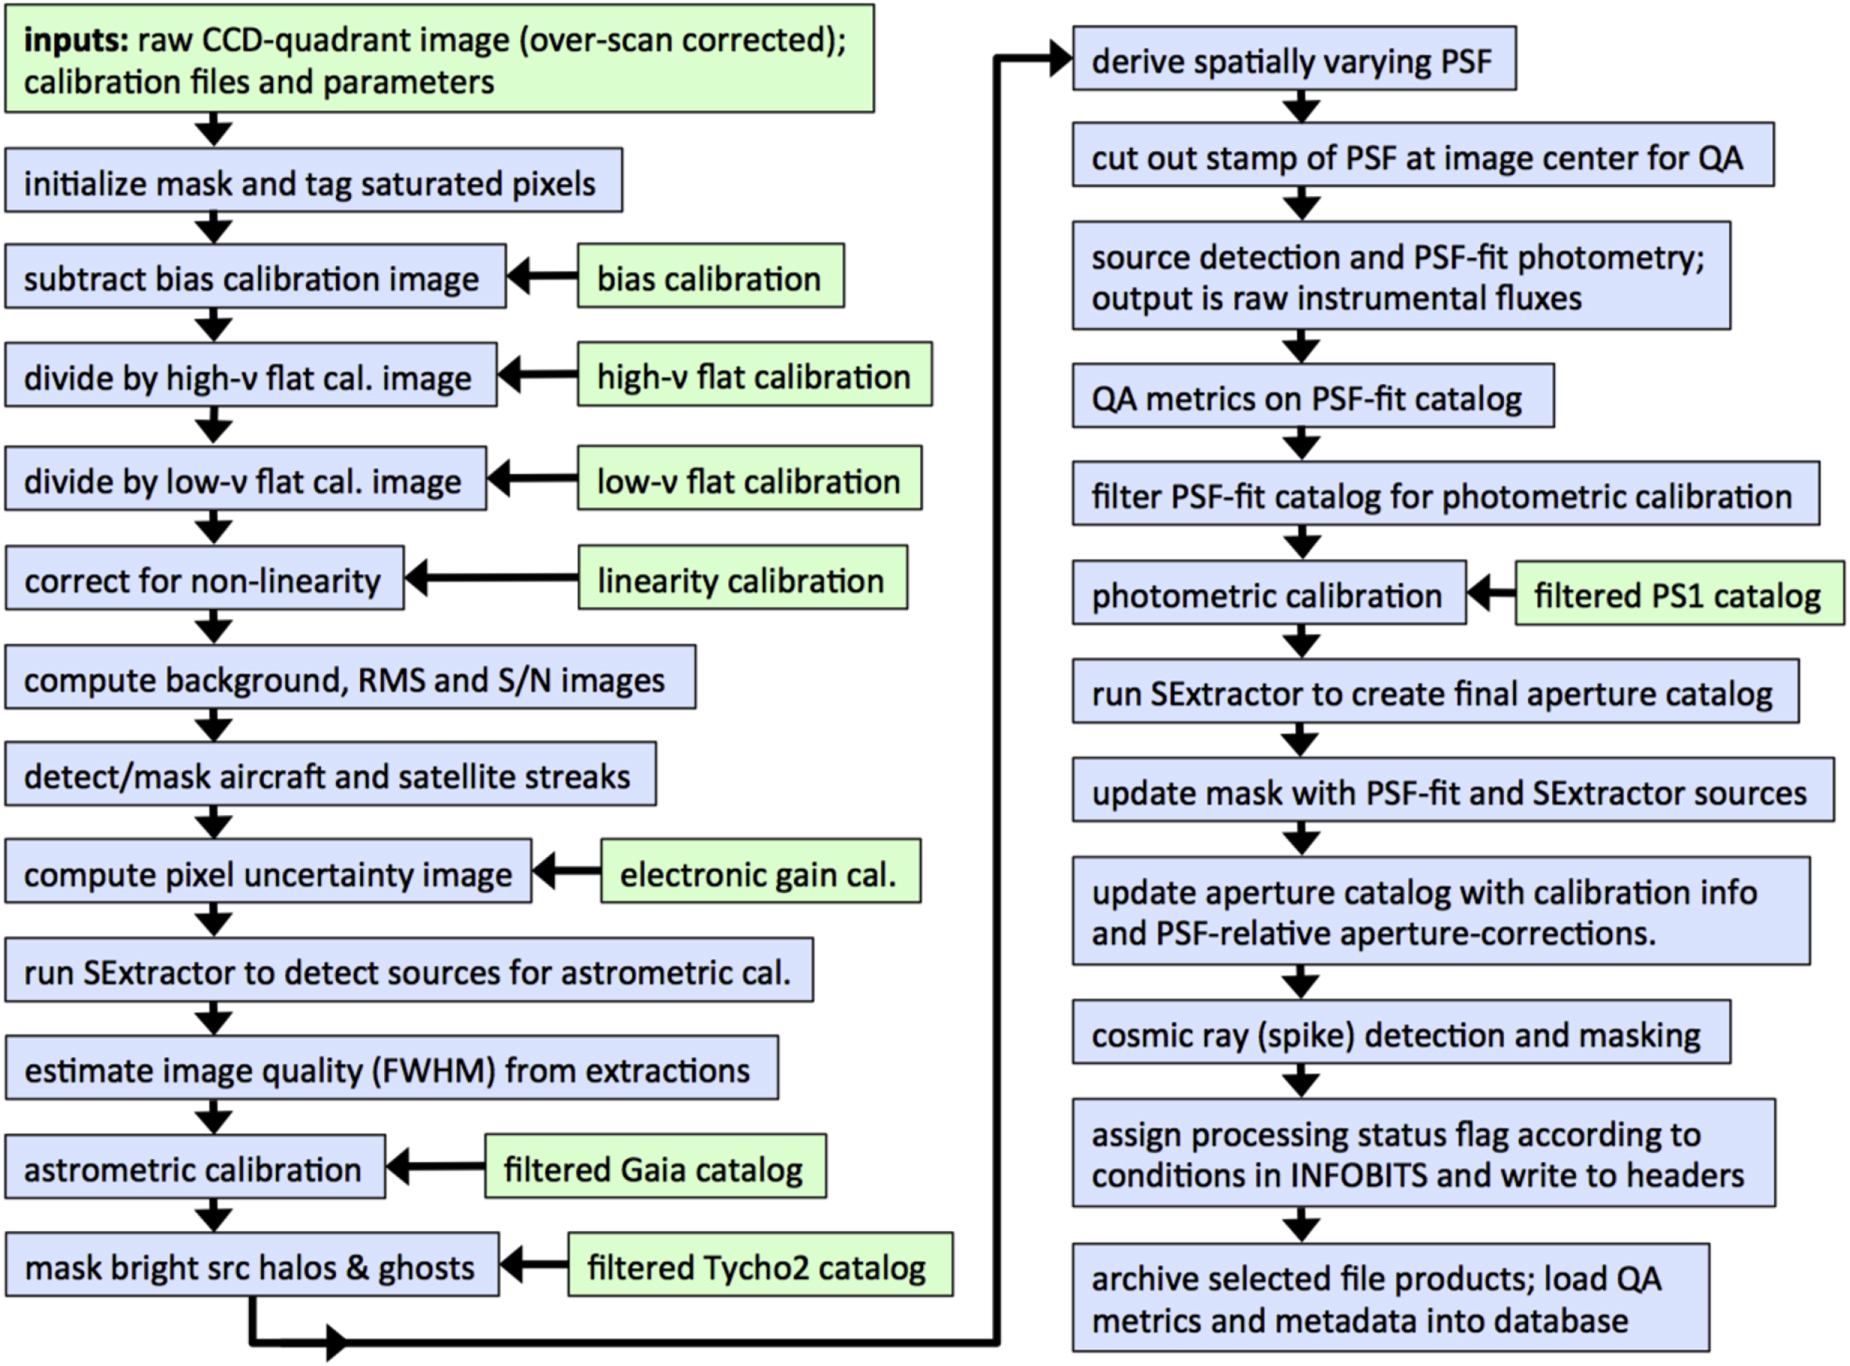
\includegraphics{ZTF/ztf_calibration}
	\caption{The full ZTF calibration process, from \cite{ztf_data_processing}.}
	\label{fig:ztf_calibration}
\end{figure}

\subsection*{Overscan Correction}

CCD cameras typically contain an \emph{overscan region}, consisting of CCD pixels at the edge of a wafer which are not illuminated by light during an exposure. These pixels provide specific calibration data for each individual exposure and quadrant, by measuring the base telescope response during a particular exposure in the absence of light. By measuring the signal in each overscan pixel, an interpolated baseline can be calculated by fitting a 2D polynomial to the overscan data \cite{ztf_data_processing}. This baseline is then subtracted from all images as a first processing step, a method known as \emph{overscan correction}. 

\subsection*{Bias Correction}

The next calibration stage involves taking overscan-corrected \emph{bias images}. These are `zero exposure' images which measure the base telescope electronics response in the absence of any integrated exposure time, providing the charge floor in each pixel. For ZTF, at least 20 such bias images are taken each night prior to observing, with these images then stacked to provide an average per-pixel bias \cite{ztf_data_processing}. A dedicated bias image is created for each CCD quadrant, and is then subtracted from all science images made that night using the CCD quadrant.

\subsection*{Flat Field Correction}

The next step is the \emph{flat field correction}, in which a known light signature is passed through the telescope, with camera performance then measured to identify any variations in response. For ZTF, there is a dedicated \emph{Flat Field Illuminator} consisting of a reflective screen inside the dome \cite{ztf_system}. This screen is illuminated by 24 LEDs, covering a range of wavelengths, enabling the detector response to be mapped across the required ZTF filters. 

%\begin{figure}[!ht]
%	\centering 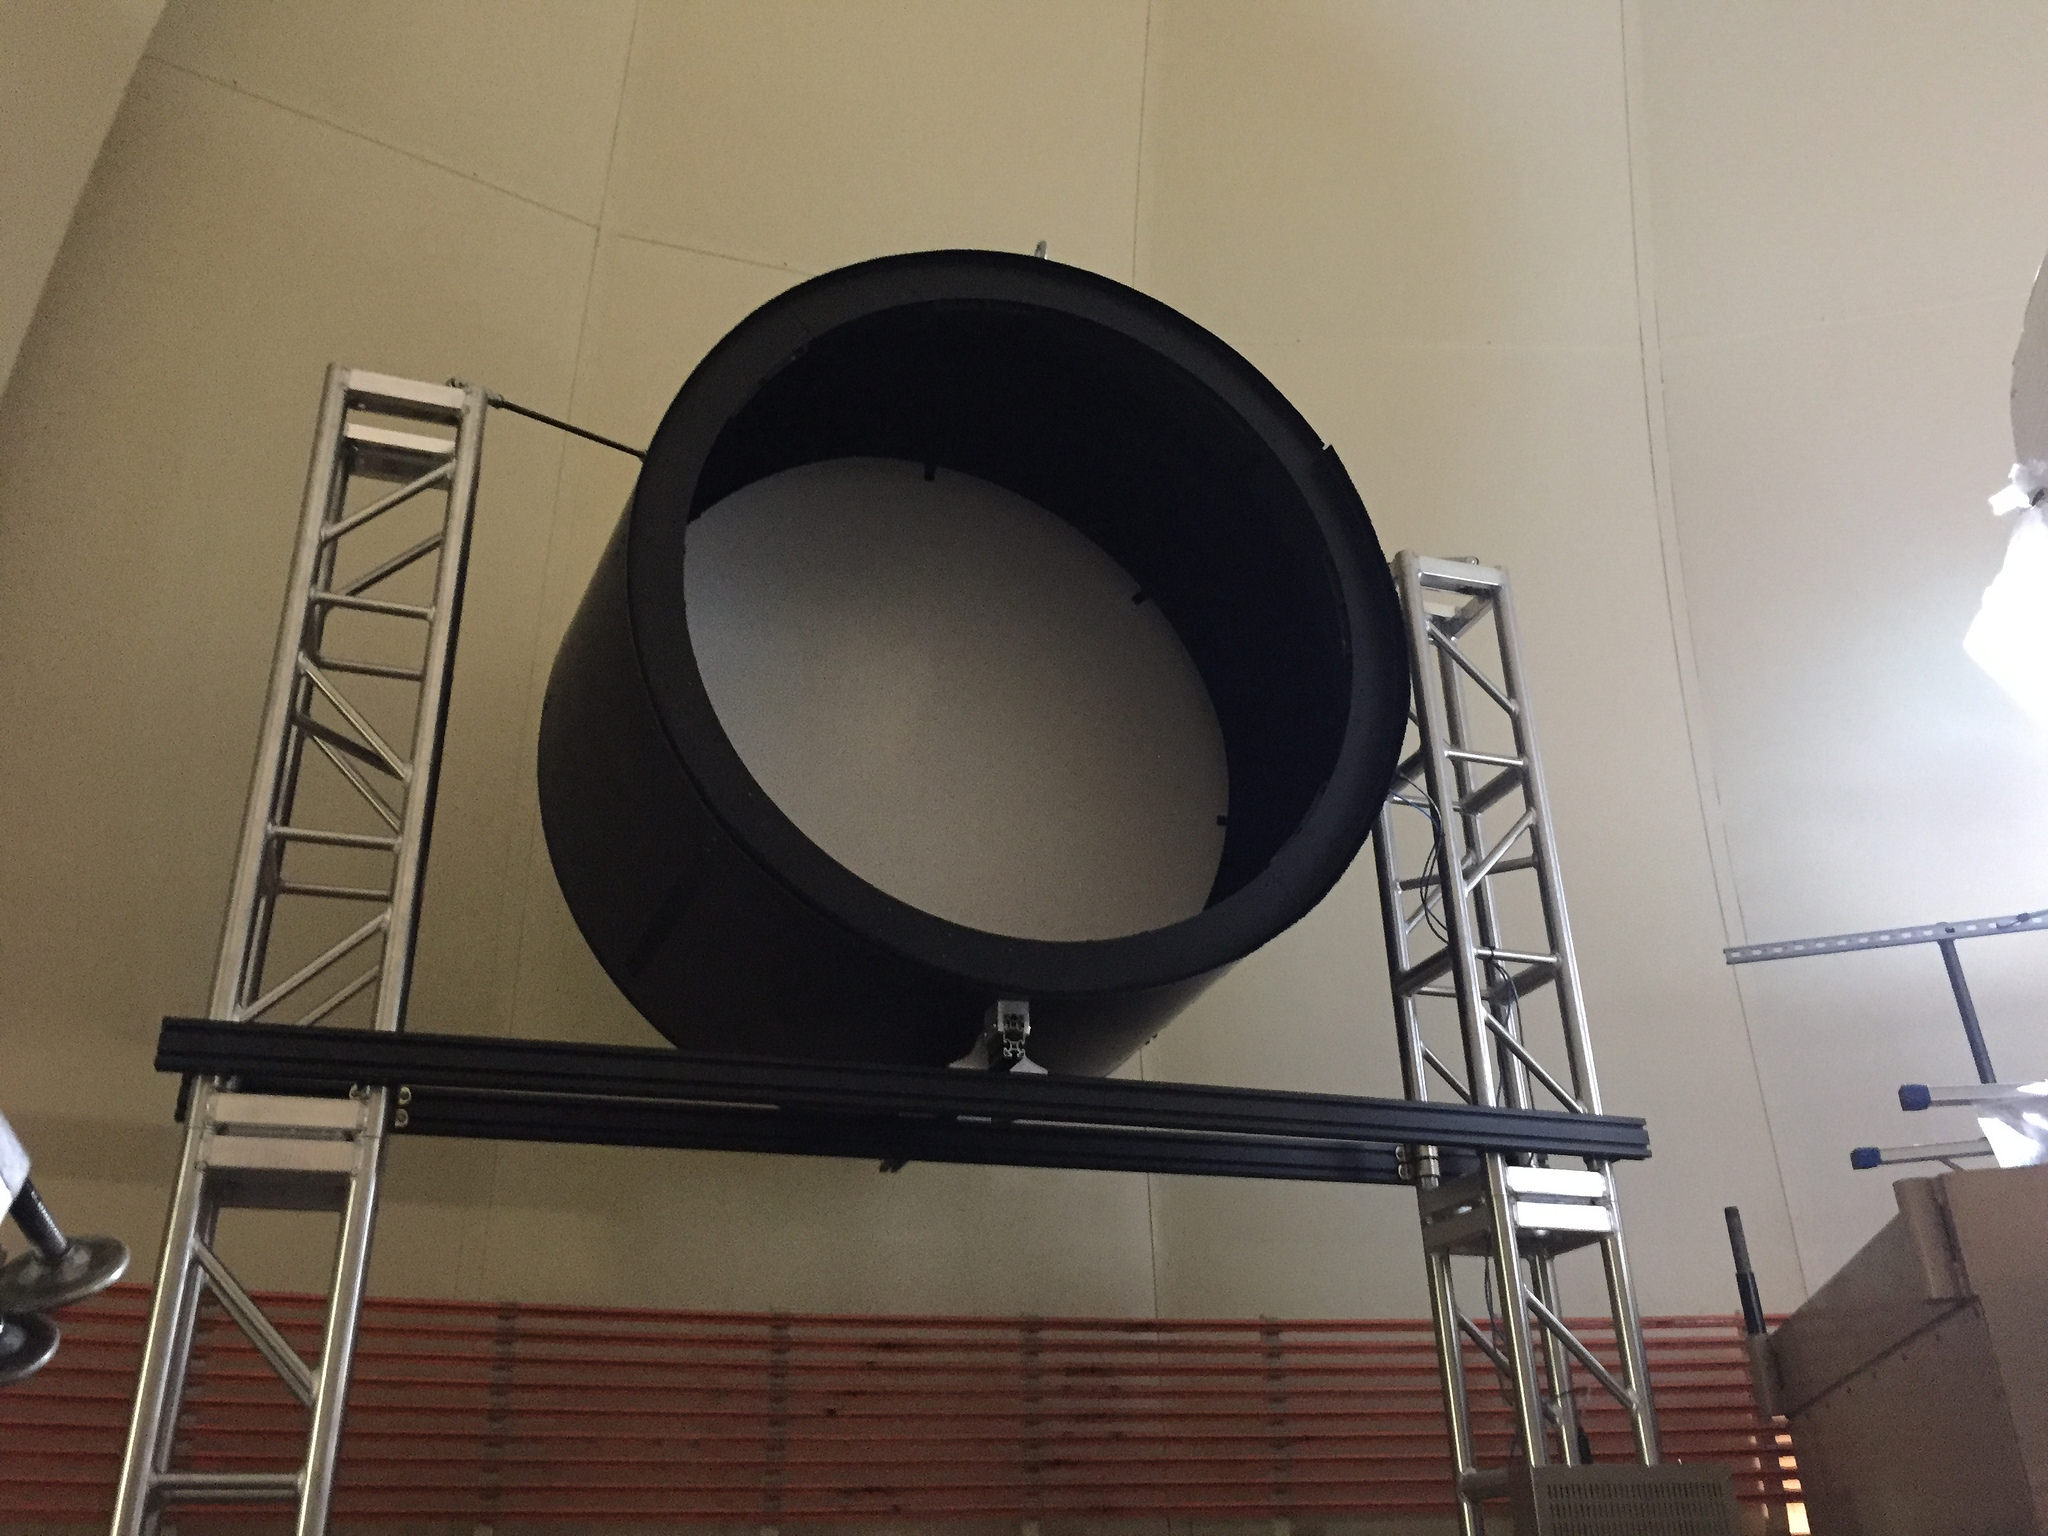
\includegraphics{ZTF/ZTF_FFI_in_dome}
%	\caption{The ZTF Flat Field Illuminator, from \cite{ztf_obs_system}.}
%	\label{fig:ztf_ffi}
%\end{figure}

New bias-corrected flat field images are taken nightly before survey operations begin, with a separate image for each quadrant and filter.  Much like for bias images, at least 20 separate images are taken and then stacked together to create the final flat field images. Each quadrant science image is then divided by the respective flat field image to normalise the response in each pixel. Systematic variations of $\sim$2.5\% have been observed between nights, and without calibration these variations would otherwise impact photometric precision \cite{ztf_data_processing}. 

\subsection*{Astrometric Calibration}

The science images must then be calibrated for \emph{astrometry}, in which the exact sky position of each telescope pixel is derived. For ZTF, this is conducted using data from the most recent \emph{Gaia} catalogue \sidecite{gaia_dr1, gaia_dr2}. \emph{Gaia} is a space-based optical survey that provides a comprehensive stellar census of the local universe, with data releases containing high-precision data on the position ($\sim$0.1 mas) and luminosity of stars with an apparent magnitude brighter than G=21 \cite{gaia_dr2}. There are $\sim$1.7 billion catalogued objects in DR2, with \emph{proper motion} also calculated for the majority of stars. Though the limiting magnitude is comparable to that of ZTF, Gaia is used for astrometric calibration because it has superior pointing accuracy due to a lack of atmospheric scattering/absorption for the satellite.

Each new ZTF science image is analysed using `source extractor' software (unfortunately named \emph{SExtractor} \sidecite{sextractor_96}), to identify sources and fit a \emph{Point Spread Function} (PSF) to each of these objects \cite{ztf_data_processing}. Bright (12 $\leq$ G $\leq$ 18) catalogued stars that have been pre-selected for each ZTF field quadrant are then matched to these sources, using the \emph{Scamp} software package \sidecite{scamp_06}. By comparing the ZTF-derived position of these stars to their `true' Gaia-derived ones, a full \emph{astrometric solution} can be found for each ZTF image, enabling a precise calibration of the sky position corresponding to each pixel in the image.

\subsection*{Photometric Calibration}

Following the calibration of positioning, images then undergo \emph{photometric calibration}. This process involves comparing the observed signal from catalogued stars to their known flux, from which the brightness of other objects can then be inferred. For photometric calibration, ZTF uses data from the first data release of the \emph{Pan-STARRs} survey (PS1) \sidecite{panstarrs_16}. Photometrically stable stars are selected (with consistent photometry across the multi-epoch PS1), with additional cuts to mitigate source confusion by excluding stars with nearby neighbours \cite{ztf_data_processing}. PS1 serves as a suitable calibration catalogue because it uses filters similar to ZTF with a substantially deeper limiting magnitude (>23 mag for g/r/i).

Much like for astrometry, the photometric calibrator star list is pre-selected for each ZTF field quadrant, with each science image then being calibrated separately based on this list \cite{ztf_data_processing}.  The calibrator list is cross matched to the sources extracted by \emph{SExtractor} in each quadrant during the astrometric calibration stage. It is assumed that the photometric bias can be parameterised as:

\begin{equation}
	m_{\textup{diff, f}} \equiv m_{\textup{PS1, f}} - m_{\textup{ZTF, f}} = ZP_{\textup{f}} + \left( c_{\textup{f}} \times PS1_{\textup{clr, f}} \right)
	\label{eq:photmetric_calibration}
\end{equation}

where f is the filter, ZP$_{\textup{f}}$ is the \emph{calibration zero point} for that filter, $c_{\textup{f}}$ is an empirical constant and $PS1_{\textup{clr, f}}$ is an estimate of the star colour from PS1 data. The $PS1_{\textup{clr, f}}$ term gives the local colour gradient, defined as the difference in apparent magnitude between the relevant PS1 filter and one adjacent filter:

\begin{itemize}
	\item ($m_{\textup{g}} - m_{\textup{r}}$) for g-band and r-band images
	\item ($m_{\textup{r}} - m_{\textup{i}}$) for i-band images
\end{itemize}

By calculating the $m_{\textup{diff, f}}$ value for all photometric calibrator stars in a quadrant, and then globally fitting these deviations to minimise $m_{\textup{diff, f}}$ using Equation \ref{eq:photmetric_calibration}, a value for the calibration zero point ZP$_{\textup{f}}$ and colour constant $c_{\textup{f}}$ can be derived for each quadrant of a science image. Having determined these values, Equation \ref{eq:photmetric_calibration} can then be used to calibrate the photometry of all other sources not included in the photometric calibrator list.

\subsection*{Image Artefacts}

ZTF images must also be corrected to remove various image artefacts, with different artefact classes targeted at specific processing stages (see Figure \ref{fig:ztf_calibration}). The following artefact classes are flagged:

\begin{itemize}
	\item\emph{Saturated pixels} are individual bright pixels that become charge-saturated, at which point they are no longer useful for image subtraction. This process provides an effective upper limit on source fluxes to which ZTF is sensitive, though variations in image quality between exposures can lead to different saturation flux thresholds \cite{ztf_data_processing}.
	\item \emph{Bad pixels} are those for which signals are untrustworthy. Some bad pixels are known in advance and masked, but further suspicious pixels with high variability are flagged through bias image analysis \cite{ztf_data_processing}. 
	\item \emph{Image streaks} can also be observed due to the movement of Near Earth Objects (NEOs) or Solar System Objects (SSOs) over the sky during an exposure. These streaks are flagged by dedicated machine learning algorithms  \sidecite{ztf_ml_19}.
	\item \emph{Ghosts} can arise from secondary reflections of bright sources in an image \sidecite{yang_02}.
	\item \emph{Cosmic rays} passing through the CCD can ionise nearby pixels, leading to a handful of bright pixels in an image.
\end{itemize}

After this stage the images are fully calibrated, and are then referred to as \emph{science images}. 

\subsection*{ZTF On-Sky Performance}

Following calibration, the 5$\sigma$ limiting magnitude can be estimated for each quadrant in a science image using a model for the detector response function and then computing the median magnitude of sources lying at the 4.5 $\leq$ S/N $\leq$ 5.5 detection threshold \cite{ztf_data_processing}. For ZTF with 30s exposures, the median limiting magnitude is 20.8 for g-band, 20.6 for r-band and 19.9 for i-band, with some dependence on the lunar cycle phase \cite{ztf_system}. The \emph{image quality} can also be derived by looking at distant sources which are intrinsically point-like, and observing the apparent spatial distribution of the corresponding flux in ZTF images, yielding a  PSF for that object. For observations above airmass 1.2, sources have a typical PSF \emph{Full Width Half Maximum} (FWHM) of 2.1\arcsec in g-band , 2.0\arcsec in r-band and 2.1\arcsec in i-band \cite{ztf_system}.

\subsection*{Reference Images}

Whereas science images provide an instantaneous view of the night sky on a given night, \emph{reference images} are created to give a comprehensive map of the static night sky baseline. By comparing science images to reference images, changes in flux from transient or variable sources can be identified. For ZTF, IPAC built reference images for each field and filter using early survey data. These reference images are composed of deep composite images containing at least 15 \emph{coadded} (stacked) individual science images taken under optimal observing conditions \cite{ztf_data_processing}. Each constituent science image was calibrated using the same processing substeps as outlined above.

\subsection*{Image Subtraction}

Much like for science images, \emph{SExtractor} source extraction is also performed on reference images to derive source PSFs. Both sets of PSFs (science and reference) are then used by the \emph{SWarp} software package \sidecite{swarp_02} to create an interpolation of the reference image projected onto the science image. The \emph{ZOGY algorithm} is then used to perform \emph{image subtraction}, where the interpolated reference image is subtracted from the science image \sidecite{zogy_16}. The resulting data product is known as a \emph{difference image}, and contains deviations between the science image and reference image arising from transient or variable sources. The threshold for a `significant detection' is set at S/N=5, with the algorithm identifying both flux increases (positive subtractions) and flux decreases (negative subtractions). 

An example of the subtraction process is shown in Figure \ref{fig:ztf_scirefdif}, based on alert data from 2018 June 19 for ZTF transient \emph{AT2018cow} (see Chapter \ref{ch:results}). The extended host galaxy is visible in both science and reference images, alongside one bright nearby object below and two additional faint objects to the right. There is a very bright excess in the science image, outshining the host galaxy, which was not present in the reference image. This can be seen even more clearly in the difference image, where a single bright gaussian-like PSF is seen. This PSF belongs to the transient, and is used to calculate the transient flux in that epoch and filter.

\begin{figure}
	\centering 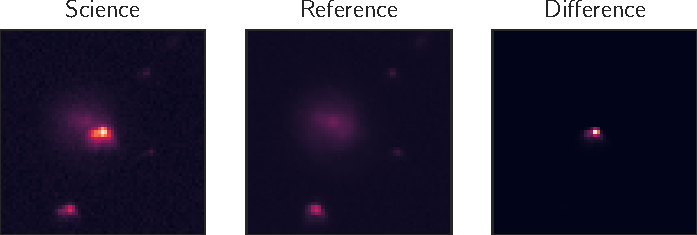
\includegraphics{ZTF/scirefdif}
	\caption{ZTF science, reference, and difference images for AT2018cow.}
	\label{fig:ztf_scirefdif}
\end{figure} 

\subsection*{Candidate Creation}

Having identified such high-significance excesses in difference images, loose quality cuts are then applied to each \cite{ztf_data_processing}. One key stage involves applying machine learning to the difference image data to assign a score for subtraction quality (the so-called \emph{RealBogus score}), enabling spurious detections arising from poor subtractions to be flagged \cite{ztf_ml_19}. Those detections passing all cuts are then formally dubbed \emph{candidates}. These new candidates are cross-matched to a database of recent candidates, linking new detections with any previous detections of the same object, and assigned a unique ZTF name if none exists. Upper limits are also calculated for recent images without significant detections of a candidate. 

Additional contextual information is found by cross-matching candidates to external catalogues such as data releases of the \emph{Gaia} or \emph{Pan-STARRs} surveys. Machine learning is also applied to determine whether nearby catalogued objects are more likely to be stars or galaxies (the \emph{StarGalaxy score}) \sidecite{ztf_stargalaxy_18}. Images are tagged by the program under which they were observed (see Section \ref{sec:survey}), to ensure consistent data access rights downstream. All of this data is then passed to the ZTF Alert Distribution System. The median duration from exposure to completed data processing is 8.5 minutes, with 90\% of detections processed within 12.6 minutes \cite{ztf_data_processing}.

\subsection*{ZTF Alert Distribution System}

The distribution of ZTF survey data is handled by the \emph{ZTF Alert Distribution System} (ZADS) \sidecite{zads_19}. ZTF ultimately detects $\sim$1 million candidates each night, with an average of $\sim$11.5 detections per image CCD quadrant \cite{ztf_data_processing}. To manage this large data volume each candidate detection is packaged as an \emph{alert} using the \emph{Apache Avro} format\footnote{\url{https://avro.apache.org}}. These alerts contain all the relevant metadata introduced above such as detection history and properties of the difference image PSF. They also contain the additional contextual data, as well as cutouts of the three calibrated images (science, reference and subtraction) such as those shown in Figure \ref{fig:ztf_scirefdif}.

 These alerts are then distributed as part of an \emph{alert stream}, to which external machines can `listen' to receive the data. Due to the size of the three images, each alert is typically $\sim$60 kB, yielding a nightly data volume of $\sim$70 GB in the alert stream.  

The original data stream transfers data from IPAC to the University of Washington (UW), where the data is then backed up \cite{zads_19}. The entire data stream is also published nightly at UW. Additional \emph{Event Brokers} can also listen to the alert stream, with these brokers being responsible for providing data access to the wider userbase. To handle differentiated data access (see Section \ref{sec:survey}) there is both a `public' stream (containing only public alerts)  and a  `partnership' stream (containing both partnership and public alerts). For this thesis, the latter stream provided the relevant data.

\section{Ampel}

For this thesis, access to ZTF data occurred primarily through \emph{Ampel}. Ampel is an open-source  software framework, developed by the ZTF groups at DESY Zeuthen and HU Berlin \sidecite{ampel}. The name refers to the initial scope of the software, handling Alert Management, Photometry and Evaluation of Light Curves (AMPEL). This Ampel software framework was used to perform the alert filtering for the \ztf ~introduced in Chapter \ref{ch:ztf_too}.

The Ampel framework is modular, performing four distinct \emph{tiers} (stages) of data processing:

\begin{itemize}
	\item \textbf{Tier 0 - Filter} - Selects the relevant alerts from a larger alert stream
	\item \textbf{Tier 1 - Update} - Identifies any corrections to apply to alert data, and crossmatches to data from any other alert streams
	\item \textbf{Tier 2 - Calculate} - Performs analysis on alert data, to calculate specific outputs
	\item \textbf{Tier 3 - Respond} - Connects the output of the analysis to the external world
\end{itemize}

For each step, the base structure is defined, with users able to contribute personalised modules based on one of these four template layers. An alert stream is provided as a starting input, which is then filtered by a Tier 0 module to select only those objects which are `interesting' for a particular science user. In principle, the alert data would then cross-matched to alert data from other instruments at the Tier 1 stage, but this is presently a theoretical step because Ampel only handles ZTF alerts. After this, any selected Tier 2 modules will be run to analyse data. Such modules could, for example, perform lightcurve analysis or cross-matching to external catalogues. Finally, this processed data is then connected to the outside world with one or more Tier 3 modules. Examples include pushing data to an external database, or pushing a high-level summary to a website. 

\begin{figure}[!ht]
	\centering 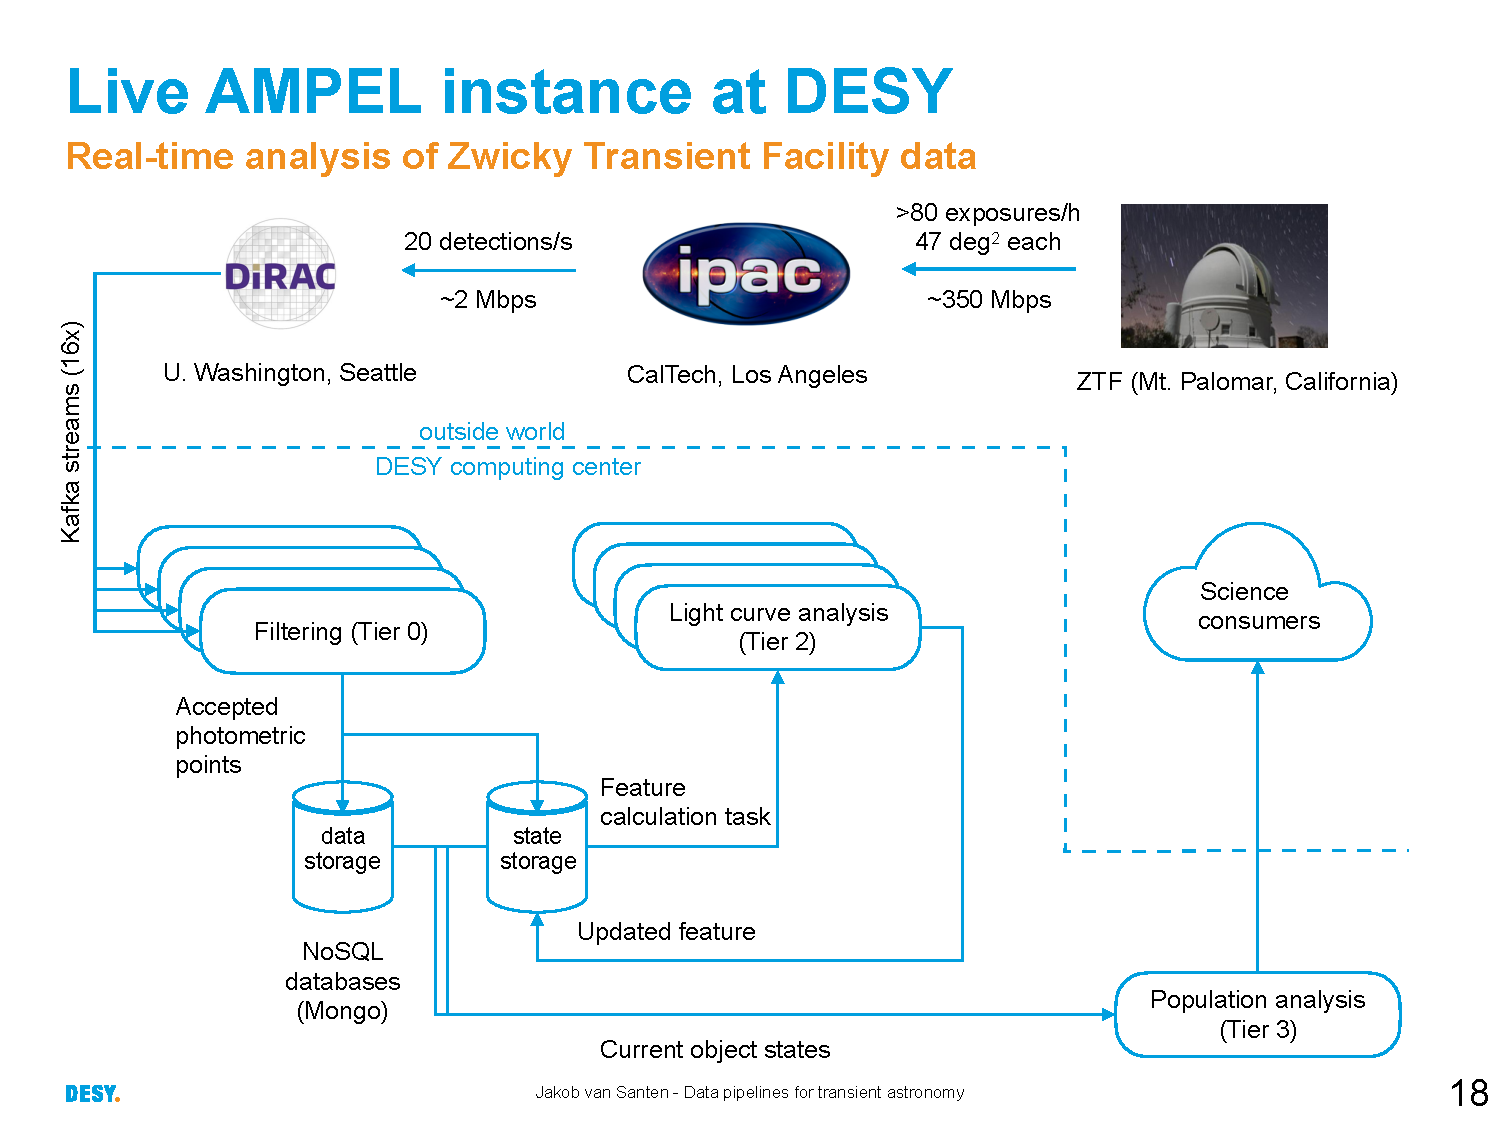
\includegraphics[trim={0 1cm 0 3cm},clip]{ZTF/ampel_intro}
	\caption{A schematic of the Ampel data pipeline, from \cite{ampel}.}
	\label{fig:ampel_pipeline}
\end{figure}

In addition to the software framework itself, the name \emph{Ampel} can also refer to the dedicated computer infrastructure running at DESY Zeuthen. As illustrated in Figure \ref{fig:ampel_pipeline}, Ampel serves as a broker, subscribing to the UW alert stream and transmitting data downstream to science users. There is a live instance of the Ampel software running at DESY that processes the ZTF partnership stream, and also hosts a number of user-defined filters from the wider collaboration. 

Of particular relevance for this thesis is the dedicated \emph{Ampel archive database}, in which all ZTF alerts are compressed and archived. The archive database can be efficiently queried by object name or spatial coordinates, providing quick access to historical ZTF data at a given position. Due to the unique selection function required for each external trigger, the \ztf ~relies on data from the archive database to `replay' old alerts. The median latency from shutter close to data availability in Ampel is under 10 minutes, though upstream delays at IPAC can increase this in some cases.
